\title{Midterm 1 for Calculus-Based Physics-1: Mechanics (PHYS150-01)}
\author{Dr. Jordan Hanson - Whittier College Dept. of Physics and Astronomy}
\date{September 25th, 2017}
\documentclass[10pt]{article}
\usepackage[a4paper, total={18cm, 27cm}]{geometry}
\usepackage{outlines}
\usepackage[sfdefault]{FiraSans}
\usepackage{graphicx}

\begin{document}
\maketitle

\section{Estimation, Approximation, and Unit Analysis}
\begin{enumerate}
\item There is a jar full of candies.  Estimate the number of candies in the jar, if this type of round candy has a radius of $\approx 0.3$ cm, and the jar has a radius of $\approx 12$ cm, and a similar height.  (Remember, the answer only has to be accurate to the correct order of magnitude).
\vspace{0.5 cm} \\
\textbf{Let the volume of the jar be $V_j$, and the volume of a candy be $V_c$.  The jar volume divided by the candy volume is the number.  $V_j / V_c = (\pi r_j^2 r_j)/((4/3)\pi r_c^3) = 3/4 (r_j/r_c)^3$.  Putting in the numbers: $(3/4)(12 cm/0.3 cm)^3 = (3/4)(120/3)^3 \approx 5 \times 10^4$.  So greater than $10^3$, but less than $10^5$.}
\vspace{0.4 cm}
\item An explorer lands on Mars, which has an acceleration due to gravity of $\approx 0.4 g$.  If the explorer drops a bag from shoulder height, how long does it take to reach the ground?
\vspace{0.5 cm} \\
\textbf{Use $\Delta x = \frac{1}{2}gt^2$, or $t = (2\Delta x/g)^{1/2}$.  Put in some numbers: $t = (2*1 m/0.4*10 m/s^2)^{1/2} = (2/4)^{1/2} s = \sqrt{1/2} s \approx 0.7 s$.  So the answer is about 0.7 seconds.}
\vspace{0.2 cm}
\item Our bodies contain special nerve fibers from the spinal cord to extermities, for quick reactions.  Suppose a curious child, who is 0.75 m tall, touches a flame.  The child's body jerks the hand away after 20 milliseconds (0.02 seconds).  What was the speed of the nerve signal? \\
\begin{itemize}
\item A: 1 m
\item B: 5 s
\item C: \textbf{20 m/s} Length of arm about length of body (more or less), divided by time.
\item D: 100 m/s (Can't be this answer, our arms are not that long).
\end{itemize}
\end{enumerate}
\section{Displacement, Velocity, and Constant Acceleration Vectors}
\begin{enumerate}
\item In the film \textit{The Hunt for Red October}, one scene depicts two Soviet officers at the helm of a submarine they are navigating through an undersea canyon.  Their current speed is 30 kilometers per hour, and the canyon turns 45 degrees to their right 1 kilometer ahead.  In how many seconds must they order the ship to turn before crashing into the side of the canyon?  After the turn, they adjust the speed to 20 kilometers per hour, and travel for 100 seconds.  What is the displacement vector from the original position?
\vspace{0.5 cm} \\
\textbf{$\Delta x = v\Delta t$, so $\Delta x/v = \Delta t = 1 km/30 km/hr = 1/30 hr = 120 sec$ for the first leg.  Then, $\Delta x = v\Delta t$ for the next leg, with $\Delta x = 20 km/hr*100s*1hr/3600s = (5/9) km$ for the second leg.  But the second leg is at a 45-degree angle to the right, starting from the end of leg 1.  If leg 1 is in the $\hat{y}$ direction, then $1 \hat{y}$ km, and leg 2 is $(5/(9\sqrt{2})\hat{x} + 5/(9\sqrt{2})\hat{y})$ km. Thus, the final displacement is $(5/(9\sqrt{2})\hat{x} + (1+5/(9\sqrt{2}))\hat{y})$ km.  Full points if you chose a different coordinate system but still get the correct corresponding displacement vector.}
\vspace{0.4 cm}
\item A torpedo is dropped in the water 1 km behind the \textit{Red October} by an overflying aircraft, and it accelerates at 3 m/s$^2$, with an initial velocity of 5 m/s.  If the \textit{Red October} does not alter course, but continues at 5 m/s, when will the torpedo reach it?
\vspace{0.5 cm} \\
\textbf{The fact that both torpedo and submarine both start with 5 m/s means that we're just interested in $\Delta x = \frac{1}{2}at^2$, with $\Delta x = 1$ km, and $a=3$ m/s$^2$.  Solving for t: $t = (2\Delta x/a)^{1/2} \approx 26$ seconds.}
\vspace{0.4 cm}
\end{enumerate}
\section{Vectors}
\begin{enumerate}
\item The astromomer Clyde Tombaugh discovered the pseudo-planet Pluto in 1930.  He observed a section of the night sky and observing the same sky one week later.  He blinked back and forth between images.  A faint star moved across the image.  Knowing how far away stars are, he concluded that the object must be inside our solar system, to be moving at a reasonable velocity.  Thus, it had to be some kind of planet.
\begin{figure}
\centering
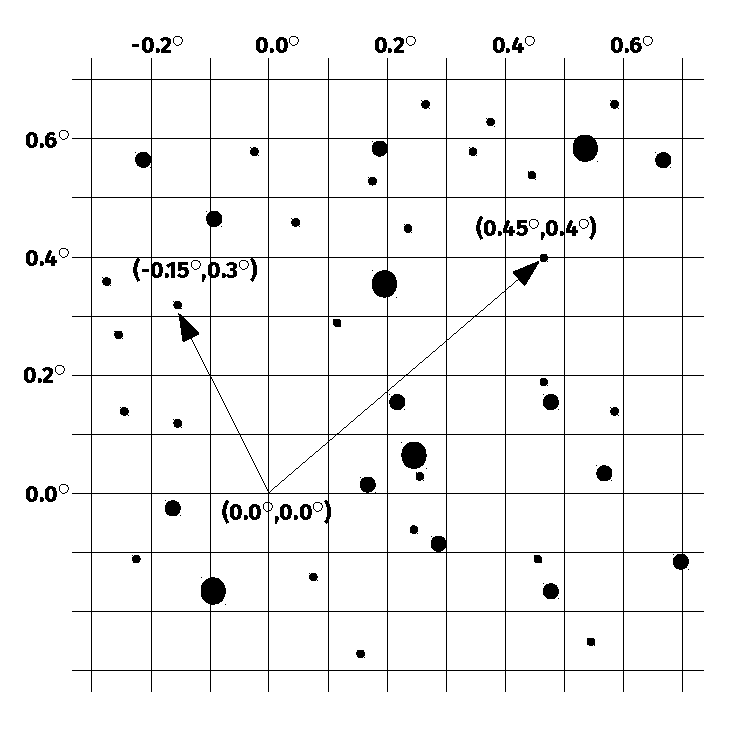
\includegraphics[width=0.5\textwidth]{PlutoDrawing.pdf}
\caption{\label{fig:1} Positions of some unknown celestial body in the solar system, circa 1930.  The vector $(-0.15^{\circ},0.3^{\circ})$ corresponds to the first observation, and the vector $(0.45^{\circ},0.4^{\circ})$ corresponds to the second observation.}
\end{figure}
a) Observe Fig. \ref{fig:1}.  Construct the displacement vector of this object, in units of degrees.  b) Construct the average velocity of this object, in units of degrees per day.  \textit{Bonus}: c) Let $s$ be the actual distance traveled, $\theta$ be the observed angle change \textit{in degrees}, and 1AU be the astronomical unit.  At the orbital radius of Pluto, $s[AU] \approx (0.02) \theta[deg]$.  How far in AU did the object move?  \textit{Bonus}: d) What is the average velocity from part c) in AU per day?  Does this answer make sense if the object is outside the solar system?
\vspace{0.5 cm} \\
\textbf{a) $\vec{x}_f = \Delta \vec{x} + \vec{x}_i$, and we have $\vec{x}_i = (-0.15^{\circ},0.3^{\circ})$, $\vec{x}_f = (0.45^{\circ},0.4^{\circ})$, and we can rearrange to get $\Delta \vec{x} = \vec{x}_f - \vec{x}_i$.  Thus $\Delta\vec{x} = (0.6,0.1)^{\circ}$. b) The vectors were observed one week apart, so $\Delta\vec{x}/\Delta t = (0.6,0.1)^{\circ}/(7 days) = (0.086,0.014)^{\circ}/day$.  c) $\Delta \vec{x} = (0.6,0.1)^{\circ} \times 0.02 AU/^{\circ} = (12,2) \times 10^{-3} AU$.  d) $(12/7,2/7) \times 10{-3} AU/day \approx 2 \times 10^{-3} AU/day$ (for the magnitude).  This speed makes sense: at that orbital radius, aren't the periods of the planets several hundred years?  So converting to years from days, we have $2 \times 10^{-3} AU/day * (400 day/year) \approx 0.8 AU/year$.}
\vspace{0.4 cm}
\end{enumerate}
\end{document}